\chapter{Contribuciones de código abierto}\label{annex:contributions}

\newcommand{\issue}[3] {
    \item ``#3'' --- GitHub #1 \#10\\
        \url{https://github.com/#1/issues/#2}
}
\newcommand{\pr}[3] {
    \item ``#3'' --- GitHub #1\\
        \url{https://github.com/#1/pull/#2}
}

% TODO: usar `emph` para issues/pull requests?

Una de mis partes favoritas del proyecto ha sido poder contribuir tanto a
diferentes dependencias de código abierto, así que he mantenido una lista de
todas las ocurrencias. Algunas colaboraciones son más importantes que otras,
pero sigue siendo una buena métrica de los resultados obtenidos. Esto no incluye
aquellos issues o pull requests que:

\begin{itemize}
    \item No contribuyeron nada (e.g., preguntas o ideas descartadas)

    \item Fueron repetitivas (e.g., tuve que realizar varios pull requests
        idénticos en Tremor cuando arreglaba problemas con Git)

\end{itemize}

Pull Requests:

\begin{itemize}
    \issue{oxalica/async-ffi}{10}{Support for \code{abi_stable}}

    \item TODO: copiar del blog

\end{itemize}

Issues:

\begin{itemize}
    \item TODO: copiar del blog

\end{itemize}

Pull requests o issues relacionados directamente con el sistema de plugins de
Tremor:

\begin{itemize}
    \item TODO: copiar del blog

\end{itemize}

Adicionalmente, aunque no esté relacionado directamente con contribuciones de
código abierto, otro logro del que me siento extrañamente orgulloso es de romper
el mismo compilador de Rust una vez, como se ve en la
Figura~\ref{fig:rustc_crash}.

TODO: a lo mejor sobra esto? A mi la verdad que me gusta

\begin{figure}
    \centering
    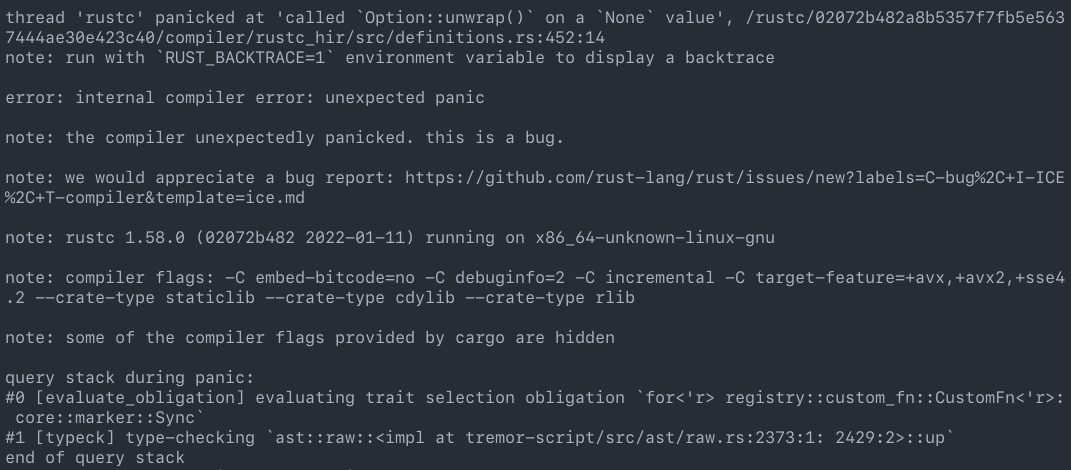
\includegraphics[width=\textwidth]{./Imagenes/rustc_crash.png}
    \caption{Error de compilación de \code{rustc}, relacionado con la
    compilación incremental y arreglado ya en una futura
    versión~\cite{rustc_fix}.}%
    \label{fig:rustc_crash}
\end{figure}
